\documentclass[9pt]{extarticle}
\usepackage[letterpaper,margin=0.46in]{geometry}
\usepackage[T1]{fontenc}
\usepackage{charter}
\usepackage{euler}
\usepackage{amsmath,amssymb,amsfonts}
\usepackage{microtype}
\usepackage{graphicx}
\usepackage{booktabs,tabularx,array}
\usepackage{xcolor}
\usepackage{fancyhdr}
\pagestyle{fancy}
\fancyhf{}
\lhead{Square--hexagon period certificate}
\rhead{Bradley Klee}
\cfoot{\thepage}
\setlength{\parindent}{0pt}
\setlength{\parskip}{4pt}
\setlength{\jot}{2pt}
\allowdisplaybreaks
\newcommand{\pa}{\partial_\alpha}
\newcommand{\QQ}{\mathbb Q}
\begin{document}

\begin{center}
{\Large\bfseries Square--Hexagon Plane-Curve Period Certificate}\\[2pt]
{\small Deductive exact reduction, reduced primitive, and replay payload}\\[3pt]
{\small Research owner: Bradley Klee --- 2 August 2026}
\end{center}

\begin{center}
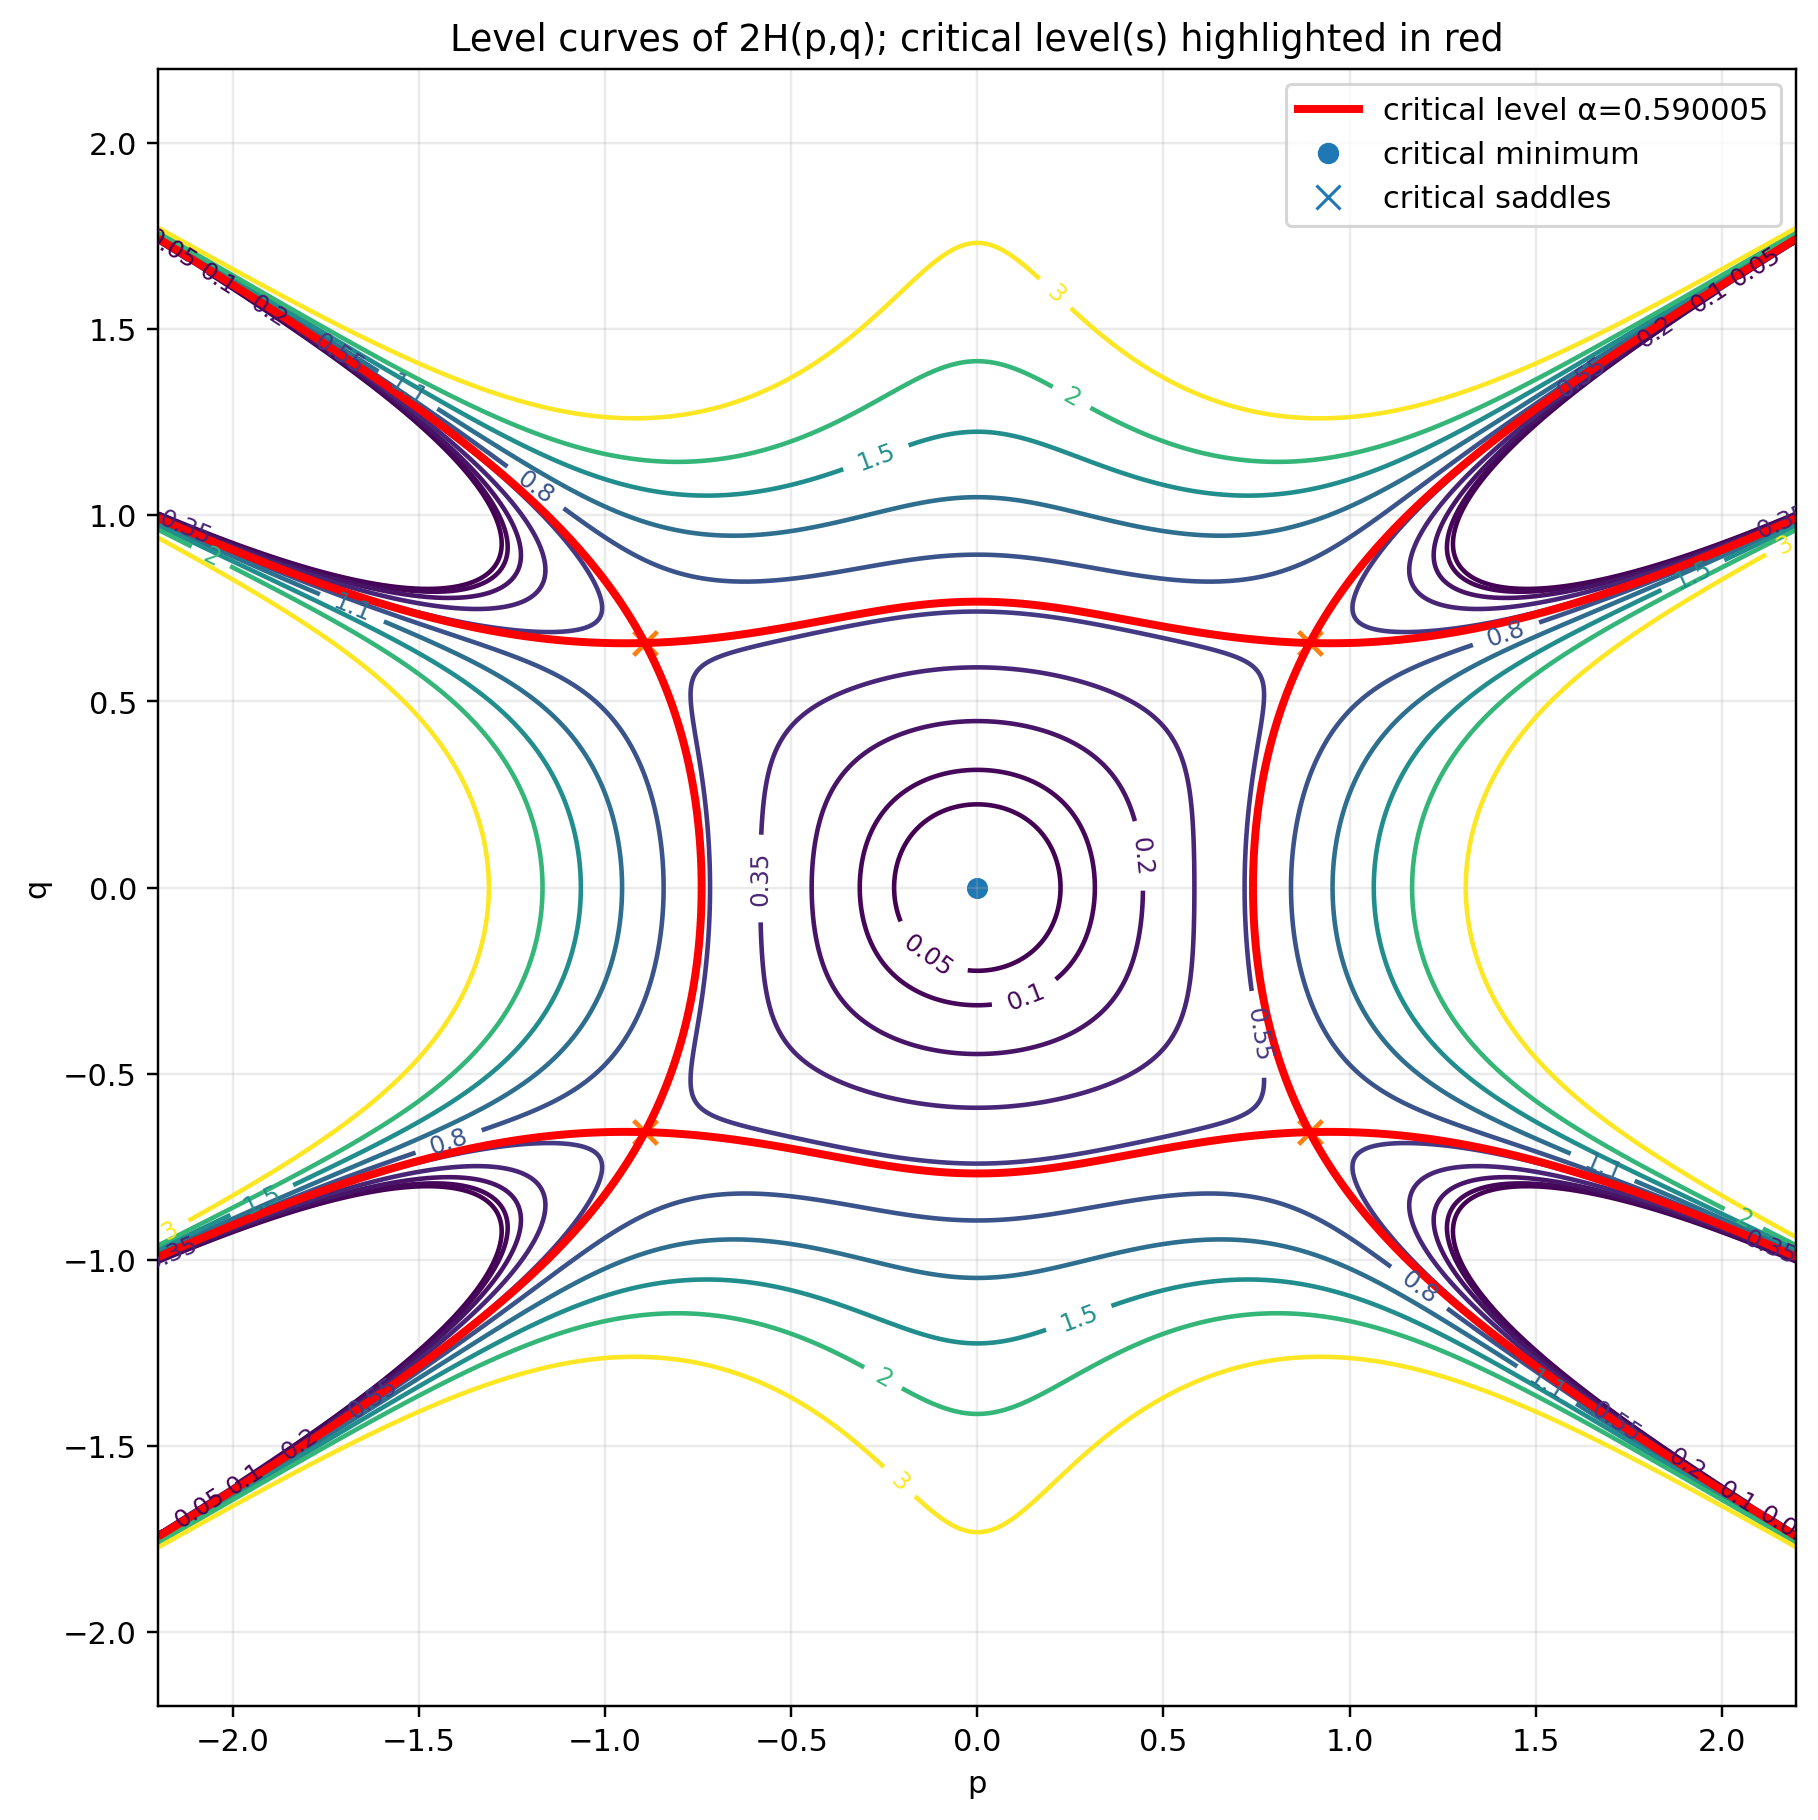
\includegraphics[width=0.70\textwidth]{assets/level_curves_with_separatrix.png}
\end{center}
\vspace{-4pt}

\begin{tabularx}{\textwidth}{@{}>{\bfseries}p{0.95in}X@{}}
Curve & $\displaystyle \alpha=2H(p,q)=p^2+q^2-2p^2q^2+\frac14p^2(p^2-3q^2)^2.$\\[6pt]
Pole & $\displaystyle \rho=(2H)_p=\frac p2(3p^4-12p^2q^2+9q^4-8q^2+4).$\\[6pt]
Period & $\displaystyle \omega=\frac{dq}{H_p}=\frac{2\,dq}{\rho},\qquad T(\alpha)=\oint_{C_\alpha}\omega,\qquad T(0)=2\pi.$\\[6pt]
Operator & $\displaystyle A_4=\sum_{j=0}^4P_j(\alpha)\pa^j.$\\[6pt]
Certificate & $\displaystyle \boxed{A_4\omega=d\Xi},\qquad \Xi=\frac{V(\alpha,p,q)}{\rho^7}.$\\
\end{tabularx}

\medskip
The numerator is symmetry-compressed as
\[
V=q\left(U_0(\alpha,q^2)+p^2U_1(\alpha,q^2)+p^4U_2(\alpha,q^2)\right),
\]
with 40 nonzero coefficient polynomials and 514 expanded terms. The full
numerator is embedded as machine-readable payload rather than printed as a
wall of coefficients.

\section*{Deductive closure}
For an order-$r$ primitive $V/\rho^{2r-1}$, set the source weight
$n=\deg_p+\deg_q$. A top-symbol minor of the exact-image map is
\[
D_r(n)=419904\,(n-(8r-3))(n-(8r-4))(n-(6r-3)).
\]
Hence all source weights above $8r-3$ vanish recursively, making the reduction
finite and exhaustive. The exact ranks are
\[
\begin{array}{c|c|c|c|c|c|c}
r&n_{\max}&\text{rows}&\text{exact cols}&\operatorname{rank}C_r&
\operatorname{rank}[C_r\mid W_r]&\dim\text{ relations}\\\hline
1&5&17&6&6&8&0\\
2&13&29&18&18&21&0\\
3&21&41&30&30&34&0\\
4&29&53&42&42&46&1
\end{array}
\]
Thus the first exact cohomology relation occurs at order four and is unique.
Fraction-free quotient reduction, without loading a guessed operator, returns
exactly the $P_j$ printed below and exactly the stored numerator $V$.

\section*{Reductive closure}
The five operator polynomials have gcd $1$. The 40 coefficient polynomials of
$V$ have gcd $1$ in $\QQ[\alpha]$, and the numerical content of $V$ is $1/2$.
Therefore the integral payload is
\[
2A_4\omega=d\left(\frac{2V}{\rho^7}\right).
\]
Moreover $V$ is not divisible by $\rho$ in
$\QQ(\alpha)[p,q]/(2H-\alpha)$. Exact Gr\"obner reduction gives
\[
\operatorname{NF}_{\langle 2H-\alpha,\rho\rangle}(V)
=\frac{15qS_8(\alpha)}{2\alpha-1}R(\alpha,q^2),\qquad R\ne0.
\]
Consequently the pole $\rho^7$ is reduced and cannot be replaced by any lower
power. The degree-eight factor $S_8$ is the apparent factor in $P_4$.

\section*{Exact order-four operator}
The leading coefficient factors as
\[
P_4=8\alpha(27\alpha^2+16)
(486\alpha^3-792\alpha^2+632\alpha-197)S_8(\alpha),
\]
where
\begin{align*}
S_8={}&2404239084\alpha^8-22448717379\alpha^7+16752988620\alpha^6
-120418068744\alpha^5\\
&-163919968272\alpha^4+178534770624\alpha^3-49764209536\alpha^2
+35868448768\alpha-20307957760.
\end{align*}

{\scriptsize
\subsection*{$P_0(\alpha)$}
\begin{align*}
P_0={}& 210322835068320\alpha^{10} - 3498482777898960\alpha^{9} + 258867849968730\alpha^{8} \\
&\quad - 25587434109688560\alpha^{7} - 151470537161887440\alpha^{6} + 236251468646553600\alpha^{5} \\
&\quad - 51572995009102080\alpha^{4} + 36074244119696640\alpha^{3} - 73265007106406400\alpha^{2} \\
&\quad + 27392394965176320\alpha - 3161055263293440.
\end{align*}

\subsection*{$P_1(\alpha)$}
\begin{align*}
P_1={}& 3654359259312060\alpha^{11} - 48803981756242707\alpha^{10} + 47241225871751484\alpha^{9} \\
&\quad - 376619237191140624\alpha^{8} - 807894950107229280\alpha^{7} + 1830637200177129888\alpha^{6} \\
&\quad - 1174507375213524096\alpha^{5} + 618762464016620544\alpha^{4} - 481098289601008128\alpha^{3} \\
&\quad + 279714899019497472\alpha^{2} - 90774194832973824\alpha + 9669720119574528.
\end{align*}

\subsection*{$P_2(\alpha)$}
\begin{align*}
P_2={}& 6265867794743700\alpha^{12} - 75876665783648193\alpha^{11} + 112112627078488392\alpha^{10} \\
&\quad - 572523884171740728\alpha^{9} - 469122498283346928\alpha^{8} + 1816134511615957152\alpha^{7} \\
&\quad - 1881625776443915328\alpha^{6} + 1326407688732674304\alpha^{5} - 771727244978217984\alpha^{4} \\
&\quad + 409283435562258432\alpha^{3} - 182117358126620672\alpha^{2} + 50849032933474304\alpha \\
&\quad - 8304120428888064.
\end{align*}

\subsection*{$P_3(\alpha)$}
\begin{align*}
P_3={}& 2523874020819840\alpha^{13} - 28801428031403280\alpha^{12} + 53737798199249664\alpha^{11} \\
&\quad - 212777881731573984\alpha^{10} - 8857742957395632\alpha^{9} + 416970391270729248\alpha^{8} \\
&\quad - 643623914923349760\alpha^{7} + 603478186349321088\alpha^{6} - 409940704413324288\alpha^{5} \\
&\quad + 219849486323659776\alpha^{4} - 105829863125549056\alpha^{3} + 42068878165671936\alpha^{2} \\
&\quad - 11665912913985536\alpha + 1536256388628480.
\end{align*}

}
\medskip
\noindent The expanded $P_4$ is omitted because the displayed factorization is exact.

\section*{Replay and embedded payload}
Run from the packet root:
\begin{verbatim}
python3 exact/verify_merged_certificate.py
python3 exact/derive_deductive_certificate.py
python3 exact/verify_reduced_primitive.py
python3 exact/verify_operator_ladder_400.py
python3 exact/verify_ore_relations.py
\end{verbatim}
Expected markers are
\texttt{MERGED\_CERTIFICATE\_PASS},
\texttt{DEDUCTIVE\_CERTIFICATE\_PASS},
\texttt{REDUCED\_PRIMITIVE\_PASS},
\texttt{OPERATOR\_LADDER\_400\_PASS}, and
\texttt{ORE\_RELATIONS\_PASS}.

The final PDF embeds the operator JSON, primitive JSON, integer-scaled
primitive, compact numerator blocks, closure witness, replay scripts, report,
and SHA-256 manifest as file attachments.

\section*{Payload manifest}
{\footnotesize
\begin{tabularx}{\textwidth}{@{}>{\ttfamily}p{1.55in}>{\ttfamily}X@{}}
SHA-256 prefix & attached file\\\hline
1bed0867cee2dd5f & exact/order4\_operator.json\\
6d778fae8e46ebbf & exact/order4\_xi.json\\
fe8cdea8eaf2bd8e & exact/order4\_xi\_integer\_scaled.json\\
0852b6fee049c119 & closure/closure\_witness.json\\
86c24f44ead7e8bc & closure/primitive\_compact.json\\
c5ea623a1f9da482 & exact/verify\_merged\_certificate.py\\
da84e1caca331780 & exact/derive\_deductive\_certificate.py\\
884172c25150cf15 & exact/verify\_reduced\_primitive.py\\
0ec10d2d79d4a396 & CLOSURE\_REPORT.md
\end{tabularx}
}

\medskip
\textbf{Scope.} The displayed identity, the order-four first-relation claim
inside the exhaustive exact reduction, and the reduced-pole claim are closed.
Coordinate changes that might beautify the operator and a conceptual
explanation of the apparent factor remain open presentation problems.

\end{document}
